\documentclass[9pt]{beamer}

\beamertemplatenavigationsymbolsempty
\renewcommand\mathfamilydefault{cmr}

\usepackage{xcolor}
\usepackage{pajmath}
\usepackage{booktabs}
\usepackage{colortbl}
\usepackage{tikz}
\usetikzlibrary{calc}
\usetikzlibrary{intersections}
\usetikzlibrary{datavisualization}
\usetikzlibrary{datavisualization.formats.functions}
\usepackage{pgfplots}

\usepackage{listings}
\usepackage{xcolor}

\definecolor{codegreen}{rgb}{0,0.6,0}
\definecolor{codegray}{rgb}{0.5,0.5,0.5}
\definecolor{codepurple}{rgb}{0.58,0,0.82}
\definecolor{backcolour}{rgb}{0.95,0.95,0.92}

\lstdefinestyle{mystyle}{
    backgroundcolor=\color{backcolour},   
    commentstyle=\color{codegreen},
    keywordstyle=\color{magenta},
    numberstyle=\tiny\color{codegray},
    stringstyle=\color{codepurple},
    basicstyle=\ttfamily\footnotesize,
    breakatwhitespace=false,         
    breaklines=true,                 
    captionpos=b,                    
    keepspaces=true,                 
    numbers=left,                    
    numbersep=5pt,                  
    showspaces=false,                
    showstringspaces=false,
    showtabs=false,                  
    tabsize=2
}

\lstset{style=mystyle}

\newcommand\VW{\V{W}}
\newcommand\bsigma{\boldsymbol{\sigma}}
\newcommand\ytrue{y^\mathrm{true}}

\title{Policy Gradient Methods}
\date{Spring 2021}

\begin{document}

\maketitle

\begin{frame}{Case Study 5, Option 2: Tic-Tac-Go}

\begin{columns}
\begin{column}{0.6\textwidth}

Your task it to write a function

\bigskip
{\small
\texttt{moveX(blocked, Xmoves, Omoves) \{} \\
\texttt{  ...}\\
\texttt{  return(nextX) \\ } 
\texttt{\}} \\}

\end{column}

\begin{column}{0.4\textwidth}
	\begin{center}
		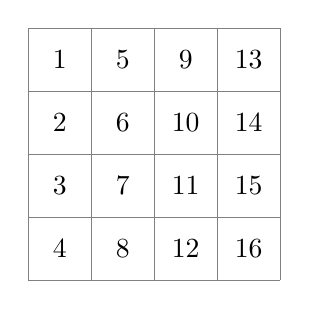
\begin{tikzpicture}[scale=0.8]
			\draw [thin,gray] (0,0) grid (4,4);
				\draw (0.5,3.5) node {1}
				(0.5,2.5) node {2}
				(0.5,1.5) node {3}
				(0.5,0.5) node {4}
				
				(1.5,3.5) node {5}
				(1.5,2.5) node {6}
				(1.5,1.5) node {7}
				(1.5,0.5) node {8}
				
				(2.5,3.5) node {9}
				(2.5,2.5) node {10}
				(2.5,1.5) node {11}
				(2.5,0.5) node {12}
				
				(3.5,3.5) node {13}
				(3.5,2.5) node {14}
				(3.5,1.5) node {15}
				(3.5,0.5) node {16};
		\end{tikzpicture}
	\end{center}	
\end{column}
\end{columns}
	
\end{frame}

\begin{frame}[fragile]{Language templates}
	\begin{lstlisting}[language=R]
		# R
		# blocked: vector of integers
		# Xmoves: vector of integers
		# Ymoves: vector of integers
		moveX <- function(blocked, Xmoves, Ymoves) {
			...
			return(nextX)
		}
	\end{lstlisting}
	
	\begin{lstlisting}[language=Python]
		# Python
		# blocked: list of integers
		# Xmoves: list of integers
		# Ymoves: list of integers
		def moveX(blocked, Xmoves, Ymoves):
			...
			return nextX
	\end{lstlisting}
	
	\begin{lstlisting}[language=Matlab]
		% Matlab
		% blocked: array of integers
		% Xmoves: array of integers
		% Ymoves: array of integers
		function [nextX] = moveX(blocked, Xmoves, Ymoves)
			...
		end
	\end{lstlisting}
\end{frame}




\begin{frame}{Implicit vs.\ Explicit Policy Methods}

\begin{itemize}
	\item So far we've used an \emph{implicit} policy for selecting actions.
	\item Given a value function $V(s)$, the optimal policy at state $s_i$ selects
	\[ \arg \max_a \mathbb{E}\left\{ r_i + V(s_{i+1}) \right\} \]
	or, for $Q$-factors,
	\[ \arg \max_a Q(s_i,a). \]
	\item<2-> This approach requires that we know $V$ or $Q$, or at least can approximate them online.
	\item<2-> Sometimes it is easier to learn an optimal policy directly.
\end{itemize}
	
\end{frame}

\begin{frame}{Policies}

\begin{itemize}
	\item Recall that a policy $\pi(a,s)$ returns the probability of selecting action $a$.
	\item Formally, the implicit policy on the previous slide was
	\[ \pi(a_i,s_i) = \begin{cases} 1 & a_i = \arg \max_a Q(s_i,a) \\ 0 & \text{otherwise} \end{cases} \]
	\item<2-> Other policies return a distribution over all possible actions, and the agent selects an action based on these probabilities.
	\item<3-> Often policies are \emph{parameterized} by a vector of tunable parameters $\theta$, i.e.\ $\pi = \pi(a,s|\theta)$.
\end{itemize}
	
\end{frame}

\begin{frame}{Policy example: The newspaper problem}

\begin{itemize}
	\item Imagine you run a small newspaper that sells papers daily at newsstands (no subscriptions).
	\item Each night you need to decide how many papers to print for the next day. If you print too many, you may lose money. If you print too few, you lose sales.
	\item<2-> Definitions:
	\begin{itemize}\addtolength{\itemsep}{0.5\baselineskip}
		\item The price of a newspaper is $p$.
		\item Each paper costs $c$ to print. (Assume $c<p$.)
		\item Each day the demand for your papers is $D$. You do not know this value ahead of time; it is a random variable.
		\item The policy to learn is $\theta$, the number of papers to print each day.
	\end{itemize}
\end{itemize}
	
\end{frame}

\begin{frame}{Learning a value for $\theta$.}

The \emph{reward} is the profit for each day:
\begin{align*}
	r &= \text{revenue} - \text{expenses} \\
	&= p\min\{\theta,D\} - c\,\theta	
\end{align*}

\pause
We can compute the stochastic gradient of the daily reward:

\[ \frac{dr}{d\theta} = \begin{cases} p-c & \text{if } \theta < D \\
 -c & \text{if } \theta > D	
 \end{cases} \]
 
 \pause
 Over time we can learn an optimal policy by stochastic steepest ascent
 \[ \theta^{(k+1)} = \theta^{(k)} + \alpha \frac{d}{d\theta}r(\theta^{(k)}) \]
 for some learning rate $\alpha$.

\end{frame}

\begin{frame}{The REINFORCE algorithm}

One of the earlier policy gradient methods was REINFORCE (Williams 1992). It is still used today for finding policies from experience.

\pause\bigskip
\begin{enumerate}\addtolength{\itemsep}{0.5\baselineskip}
	\item Initialize the policy parameters $\theta$, possibly to random values.
	\item Generate a trajectory $s_0,a_0,r_0,\,\ldots,s_{T-1},a_{T-1},r_{T-1},\,s_T,r_T$.
	\item foreach $i\in \{0,\ldots,T\}$:
		\begin{itemize}\addtolength{\itemsep}{0.5\baselineskip}
			\item Calculate the return $R_i = r_i + r_{i+1} + \cdots + r_T$.
			\item $\theta \leftarrow \theta + R_i\nabla_\theta \log \pi(a_i,s_i|\theta)$
		\end{itemize}
	\item Go to step \#2 and repeat.
\end{enumerate}
	
\pause
\bigskip
Note that the policy $\pi$ can be any parameterized function, including a neural network. The details of the parameter update change based on the structure of $\pi$, e.g.\ by using backpropagation.

\end{frame}

\begin{frame}{Summary}

\begin{itemize}\addtolength{\itemsep}{0.5\baselineskip}
	\item Policy gradient methods learn policies directly from experience.
	\item Stochastic search methods can find simple policies, and REINFORCE works well for complex policies.
	\item<2-> \textbf{Next time:} AlphaGo has a value network, a policy network, and tree search (rollout). How do these all fit together?
\end{itemize}
	
\end{frame}



\end{document}
